\documentclass[a4paper]{article}
%\usepackage[ngerman]{babel}
\usepackage[T1]{fontenc}
\usepackage[utf8]{inputenc}
\usepackage{textcomp}
\usepackage{geometry}
\geometry{ left=2cm, right=2cm, top=2cm, bottom=3cm, bindingoffset=5mm}
\usepackage{graphicx}
\usepackage{xcolor}
\usepackage{hyperref}
\usepackage{longtable}
\usepackage{amstext}
\usepackage{array}
\usepackage{amsmath}
\newcolumntype{L}{>{$}l<{$}}
\usepackage{tabularx, ragged2e}
\usepackage{helvet}
\renewcommand{\familydefault}{\sfdefault}
\usepackage{lastpage}
\usepackage{todonotes}
\usepackage{titlesec}
\titleformat*{\section}{\large\bfseries}
\usepackage{listings}
\usepackage{color}

\usepackage{tikz}
%\newcommand{\tikzmark}[2]{\tikz[overlay, remember picture] \node[inner sep=0pt, outer sep=0pt, anchor=base] (#1) {#2};}
\usetikzlibrary{tikzmark}


\definecolor{mygreen}{rgb}{0.18, 0.545, 0.341}
\definecolor{mygray}{rgb}{0.5,0.5,0.5}
\definecolor{myblue}{rgb}{0.53,0.61,0.85}

\lstset{
 keywordstyle=\color{mygreen},
 commentstyle=\color{mygray},
 numbers=left,
 numbersep=5pt, 
 numberstyle=\scriptsize\color{mygray}
 }

\usepackage{amsmath,amssymb}

\DeclareRobustCommand{\bbone}{\text{\usefont{U}{bbold}{m}{n}1}}

\DeclareMathOperator{\EX}{\mathbb{E}}% expected value

\date{}
\author{}
\usepackage{fancyhdr}
\pagestyle{fancy}
\fancyhf{}
\fancyhead[R]{Felix Burk\\ Pascal Huszár}
\fancyhead[L]{Reinforcment Learning \\ Summer Term 2021 }
\fancyfoot[R]{page \thepage \text{ }/ \pageref*{LastPage}}
%\fancyfoot[LE]{Seite \thepage \text{ }von \pageref{LastPage}}
\renewcommand{\headrulewidth}{0.5pt}

\usepackage{amsmath}
\DeclareMathOperator*{\argmax}{arg\,max}
\DeclareMathOperator*{\argmin}{arg\,min}


\title{\textbf{Exercise 05}}

\begin{document}
	\maketitle 
	\thispagestyle{fancy}
    \section*{Task 1 - Random Walk}
    In the first episode the agent starts in state A and subsequently lands in the terminating state on the left, resulting in a reward of zero. Because the agent reached a terminating state the random walk is over. \\

    $V(A_1) = V(A_1) + \alpha * [R_{t+1} + \gamma*V(A_{t+1})-V(A_1)]$ \\
    
    $V(A_1) = 0.5 + 0.01 * [0 + 0 - 0.5] = 0.45$ \\
    
    The estimate for A changed by 0.05.\\
    
    \section*{Task 2 - Sarsa and Q-learning on the FrozenLake}
    \subsection*{a)}
    \begin{center}
    	\begin{tabular}{ c c c c }
			↓ & ↑ & ↓ & ↑ \\ 
			← & ← & → & ← \\
			↑ & ↓ & ← & ← \\
			← & ↓ & → & ←   
    	\end{tabular} \\\vspace{10pt}
        	Sarsa policy 
    \end{center}
\begin{figure}[!ht]
	\centering
	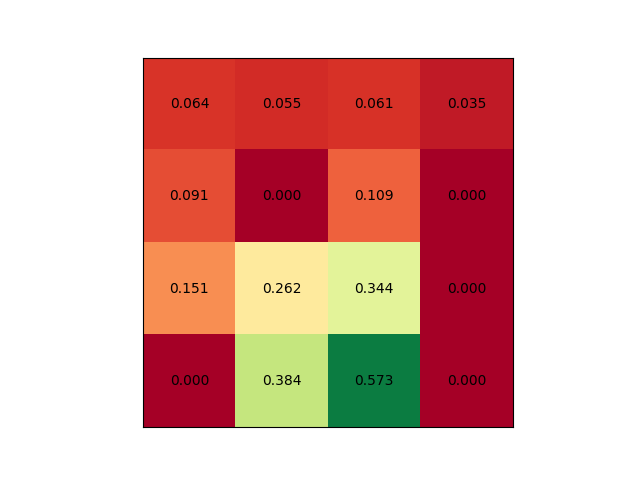
\includegraphics[width=0.8\linewidth]{state_value_sarsa}
	\caption{State value -  Sarsa }
	\label{fig:state_value_sarsa}
\end{figure}
\begin{figure}[!ht]
	\centering
	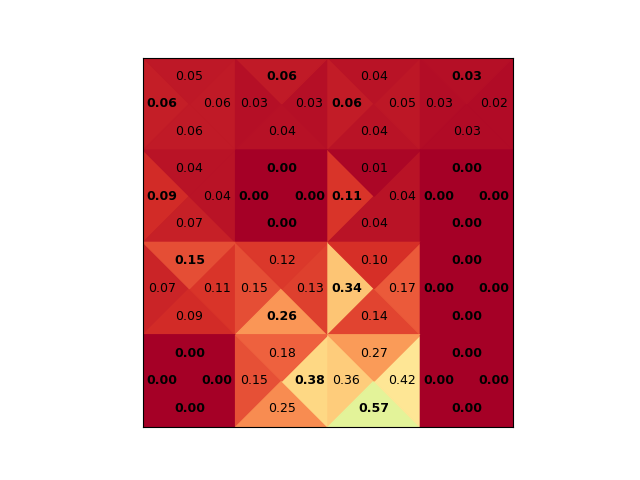
\includegraphics[width=0.8\linewidth]{action_value_sarsa}
	\caption{Action value - Sarsa}
	\label{fig:action_value_sarsa}
\end{figure}

\newpage
\subsection*{b)}
\begin{center}
	\begin{tabular}{ c c c c }
		→ & ↑ & ↓ & ↑ \\ 
		← & ← & → & ← \\
		↑ & ↓ & ← & ← \\
		← & → & ↓ & ←  
	\end{tabular} \\\vspace{10pt}
	Q-Learning policy
\end{center}

\begin{figure}[!ht]
	\centering
	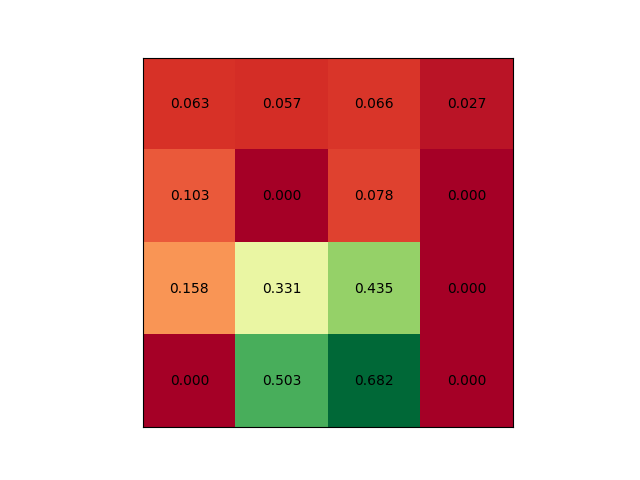
\includegraphics[width=0.8\linewidth]{state_value_qlearning}
	\caption{State value -  Q-Learning }
	\label{fig:state_value_qlearning}
\end{figure}
\begin{figure}[!ht]
	\centering
	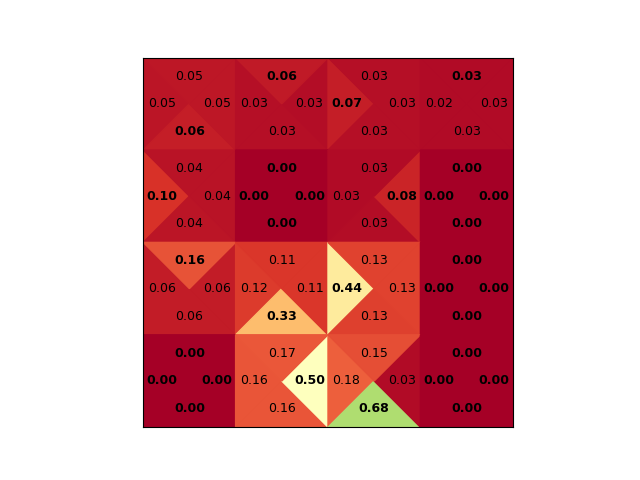
\includegraphics[width=0.8\linewidth]{action_value_qlearning}
	\caption{Action value - Q-Learning}
	\label{fig:action_value_qlearning}
\end{figure}

\newpage
\subsection*{c)}
    \begin{center}
	\begin{tabular}{ c c c c }
		↓ & → & ↓ & ↓ \\
		↓ & ← & ↓ & ← \\
		→ & ↓ & ← & ← \\
		← & → & → & ←  
	\end{tabular} \\\vspace{10pt}
	Det. Sarsa policy 
\end{center}
\begin{figure}[!ht]
	\centering
	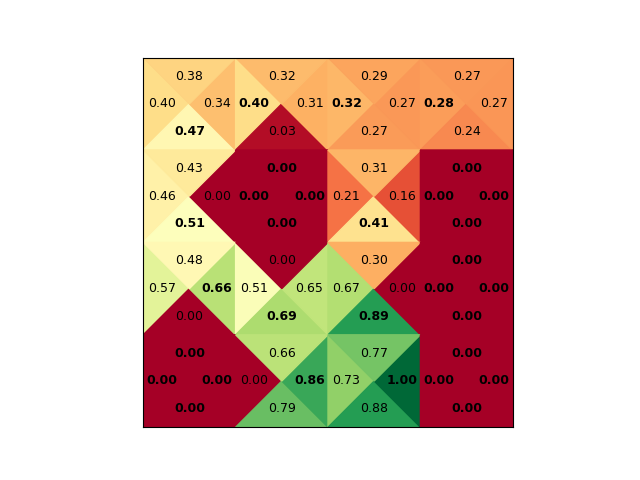
\includegraphics[width=0.8\linewidth]{det_action_value_sarsa}
	\caption{DET: Action value - Sarsa}
	\label{fig:action_value_qlearning}
\end{figure}

\newpage
\begin{center}
	\begin{tabular}{ c c c c }
		→ & → & ↓ & ↑ \\ 
		↑ & ← & ↓ & ← \\
		↑ & ↑ & ↓ & ← \\
		← & ↓ & → & ← 
	\end{tabular} \\\vspace{10pt}
	Det. Q-Learning policy 
\end{center}
\begin{figure}[!ht]
	\centering
	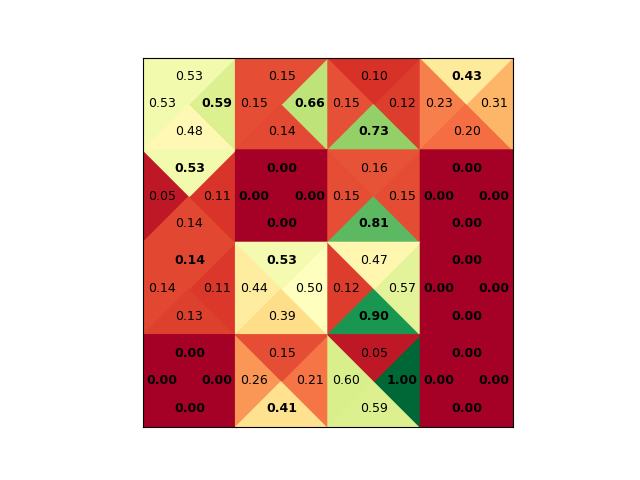
\includegraphics[width=0.8\linewidth]{det_action_value_qlearning}
	\caption{DET: Action value - Q-Learning}
	\label{fig:action_value_qlearning}
\end{figure}

\newpage
\subsection*{d)}
	For the larger FrozenLake environment, uncomment: \\
	
	env=gym.make('FrozenLake-v0', map\_name="8x8")
\end{document}